\chapter{Cobertura de la demanda. Mercado eléctrico.}
\section{Explotación del mercado eléctrico.}
La energía eléctrica se genera en grandes concentradas de forma concentrada y posteriormente se transmite a grandes distancias donde el equilibrio se obtiene de las curvas de oferta y demanda.


Una misión importante de la red es la de ajustar la energía generada a la demandada con unos valores de tensión (Control Q-U) y frecuencia (Control P-f).
\section{Curva de demanda diaria.}
La demanda varia constantemente tanto hora a hora como diariamente. Esta demanda se refleja en las curvas de carga o demanda donde la diferencia entre ambas equivale a las pérdidas en la red ($\approx$12\%).

\begin{itemize}
	\item [-]\textbf{Energía producida:} se entiende en barras de la central, descontando el autoconsumo.
	\item [-]\textbf{Energías consumida:} se obtiene de la suma del consumo de los abonados.
\end{itemize}
\begin{figure}[H]
	\begin{minipage}{0.5\linewidth}
		\centering
		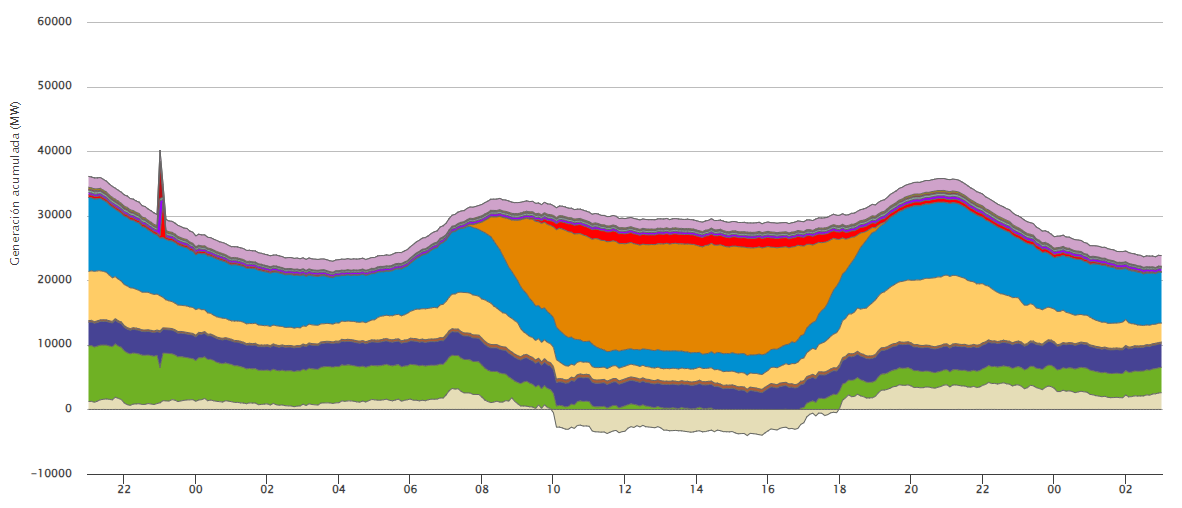
\includegraphics[width=0.7\linewidth]{res/tema4/demandaDia}
		\label{fig:demandadia}
	\end{minipage}
	\begin{minipage}{0.5\linewidth}
		\centering
		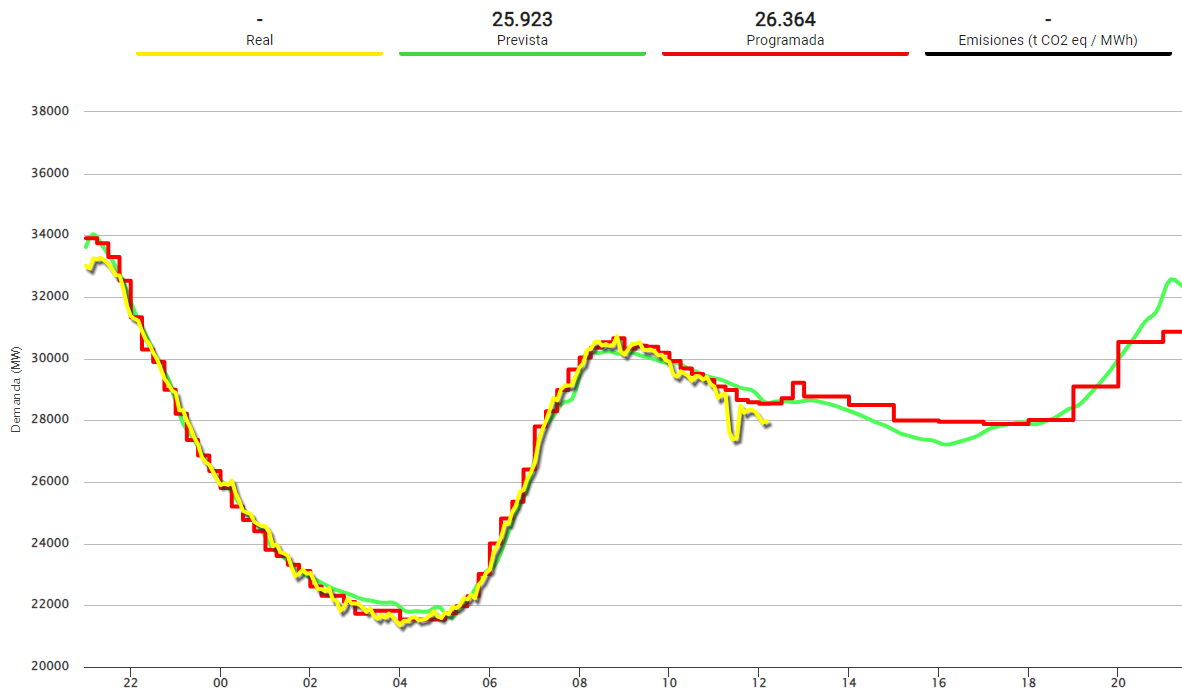
\includegraphics[width=0.7\linewidth]{res/tema4/demandaDia1}
		\label{fig:demandadia1}
	\end{minipage}
\end{figure}
La curva de carga o de demanda se predice mediante la estadística acumulada de muchos años ya que para fijar el precio es necesaria esta previsión (tiene un error asociado del 2\%). En estos datos, se pueden apreciar típicamente tres picos de consumo (12, 16 y 20 horas) que llevan a la tarifa PVPC (Precio de venta al pequeño consumidor) con discriminación horaria en horas valle, llano y punta.


Cabe destacar, como los factores locales tienen mucho peso sobre la demanda real como la temperatura, grandes eventos, ...

\section{Pérdidas en la red.}
Son un coste de operación necesario para mover la energía desde donde se produce (Galicia y Cataluña como pozos) hacia donde se consume (Madrid y Barcelona como sumideros). 
\begin{itemize}
	\item [-] Red de transporte 1-2\%
	\item [-] Red de distribución 4-6\%
	\item [-] Red baja tensión 7-10\%
\end{itemize}
\section{Gestión de la red.}
La empresa encargada de la gestión de la red es Red Eléctrica Española (REE) que recibe a través de su red de fibra óptica las potencias activa y reactiva en varios puntos de la red. La gestión se realiza desde el Centro de Control Eléctrico (CECOEL).

Para realizar esta gestión REE debe tener en cuenta muchas incertidumbres asociadas a defectos en generadores y la red lo cual provoca un sobredimensionamiento del sistema.
\subsection{Incidencias no previstas.}
Cuando ocurren incidencias graves, normalmente asociadas a una falta en la generación REE debe aplicar cortes a las industrias acogidas a contratos de interrumpibilidad.
\subsection{Configuración sistema eléctrico de potencia.}
El sistema léctrico de potencia se compone de lo siguientes elementos:
\begin{itemize}
	\item [-] \textbf{Generación:} Se genera en barras del generador de 6-30 kV a 50Hz con potencias de hasta 1500 MVA.
	\item [-] \textbf{Redes de Transporte:} Esta formada por un elevado número de nodos con topología mallada a los que se conectan los generadores y consumidores a una tensión de 220-400kV.
	\item [-] \textbf{Redes de Distribución:}  Las longitudes de estas líneas no superan los 25 km y normalmente son aéreas. En núcleos urbanos suelen ser malladas y en zona rural radiales. Se distribuye de 132-15kV.
	\item [-] \textbf{Centros de transformación:} Se reduce la tensión de media a baja tensión.
	\item [-] \textbf{Consumidores:} Red de distribución a 230/400V.
\end{itemize}
\section{Funcionamiento del mercado eléctrico.}
Desde la Ley 54/1997 se liberalizó el sector eléctrico para permitir la libre competencia con las siguientes características:
\begin{itemize}
	\item [-] Libertad de construcción de nuevas centrales de producción de electricidad.
	\item [-] Competencia entre las empresas productoras de electricidad en un mercado de ofertas.
	\item [-] Libertad progresiva de los consumidores para elegir el suministrador que deseen y acordar con
	él las condiciones y precio del kWh.
	\item [-] Libertad de comercialización de la electricidad.
	\item [-] Libertad de comprar o vender electricidad a empresas y consumidores de otros miembros de
	la UE.
	\item [-] Separación jurídica de actividades:
	\begin{itemize}
		\item \textbf{Reguladas:} transporte, distribución y gestión del sistema.
		\item \textbf{No reguladas:} generación y comercialización
	\end{itemize}
	\item [-] Sostenibilidad económica y financiera:
	\begin{itemize}
		\item Garantizar el suministro al mínimo coste.
		\item Retribución de actividades con base en criterios objetivos, transparente y homogéneos.
		\item Marco normativo que garantice la estabilidad financiera.
		\item  Actualización de los peajes de acceso a través de cargos.
	\end{itemize}
\end{itemize}
La explotación del Mercado Ibérico Eléctrico (MIBEL) se realiza conjuntamente entre:
\begin{itemize}
	\item El operador del Mercado Ibérico Eléctrico (OMIE) encargado de la gestión económica.
	\item Red Eléctrica de España (REE) encargada de la gestión técnica.
\end{itemize}
En el MIBEL se fijan los precios basandose en el punto de equilibrio entre el sistema de oferta de ventas (generadores) y el sistema de oferta de compras (consumidores).
\newpage
\begin{figure}[H]
	\centering
	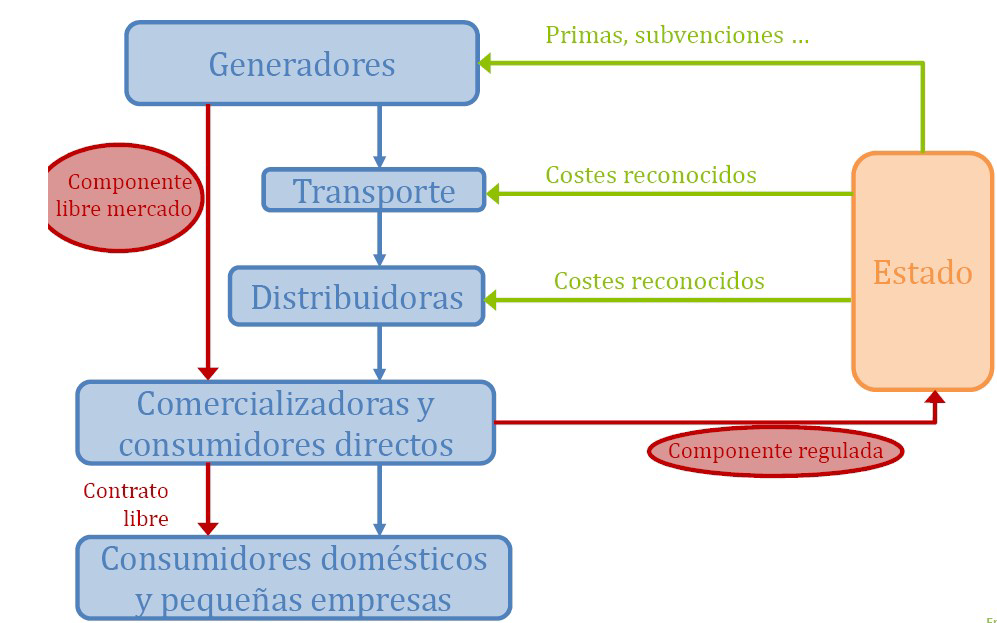
\includegraphics[width=0.7\linewidth]{res/tema4/diagramaPochoAdrikun}
	\label{fig:diagramapochoadrikun}
\end{figure}


\subsection{Actividades principales.}
Se distingue entre actividades reguladas y liberalizadas.


Actividades reguladas:
\begin{itemize}
	\item [-] \textbf{Transporte:} La única empresa encargada de esta actividad es REE. Actividad retribuida de forma regulada y sometida a planificación Estatal.
	\item [-] \textbf{Gestión técnica y económica:} La Comisión Nacional de los Mercados y la Competencia (CNMC) vigila que en las actividades liberalizadas existe competencia efectiva. Para llevar a cabo esta labor se apoya en operador de mercado (OMIE) y en el operador del sistema (REE).
	\begin{itemize}
		\item \textbf{Operador del mercado (OMIE):} Es una sociedad mercantil (con limitaciones de participación) que asume la gestión del sistema de ofertas de compra y venta de energía eléctrica. Se financia a través de precios fijados a los generadores. Cumple las siguientes funciones:
		\begin{itemize}
			\item La recepción de ofertas de compra y venta.
			\item La recepción y gestión de las garantías.
			\item Realizar la casación entre oferta y demanda (hallar el punto de equilibrio).
			\item Determinación de los precios de la energía.
			\item La liquidación de los pagos.
			\item Informar sobre la evolución del mercado.
		\end{itemize}
		\item \textbf{Operador del sistema (REE):} Es una sociedad mercantil (con limitaciones de participación) que garantiza la calidad y continuidad del sistema eléctrico. Se financia a través de precios fijados a los generadores. Cumple las siguientes funciones:
		\begin{itemize}
			\item El programa base diario de funcionamiento (cuanta demanda y oferta hay).
			\item El programa diario viable (tras aplicar las restricciones).
			\item La programación horaria final.
			\item La gestión de desvíos.
		\end{itemize}
	\end{itemize}
\end{itemize}

Actividades liberalizadas:
\begin{itemize}
	\item [-] \textbf{Producción:} Su función es operar y mantener las instalaciones de producción. Pueden ser nacionales o externos.
	
	
	La entrada de nuevos grupos esta liberalizada pero sometida a autorización reglada.
	
	
	Son el grupo encargado de realizar el sistema de ofertas en el mercado diario. Además, parte de sus ingresos viene por prestar el servicio de ajuste o reserva (lidiar con demanda no prevista).
	
	
	Actualmente, parte de la producción se realiza a partir de fuentes renovables que tienen las siguientes características:
	\begin{itemize}
		\item Limite de potencia del 40\% de la red.
		\item Venta de energía a coste 0 en el mercado diaria.
		\item Retribución basada en los ingresos del mercado y una retribución regulada:
		\begin{itemize}
			\item Retribución a la inversión.
			\item Retribución a la operación basada en la diferencia entre los costes e ingresos de explotación.
		\end{itemize}
	\end{itemize}
	\item [-] \textbf{Distribución:} Son responsables de la explotación, mantenimiento, desarrollo de su red y sus interconexiones con
	otras redes. La actividad esta retribuida de forma regulada y se pueden utilizar a cambio de un peaje. 
	
	
	En España, la península esta repartida entre Iberdrola, el grupo Naturgy y Endesa teniendo un oligopolio sobre el mercado aunque a nivel legal sea una actividad de libre competencia.
	
	
	\item [-] \textbf{Comercialización:} Acceden a las redes de distribución para vender energía a los consumidores. Pueden ser:
	\begin{itemize}
		\item De referencia: ofrecen el Precio Voluntario para el Pequeño Consumidor (PVPC). Son compañías energéticas designadas por el Ministerio de Industria, Turismo y Comercio.
		\item De mercado libre: venden a los consumidores con una potencia contratada superior a 10 kW  que están obligados a acogerse a este tipo de tarifa.
	\end{itemize}
\begin{figure}[H]
	\centering
	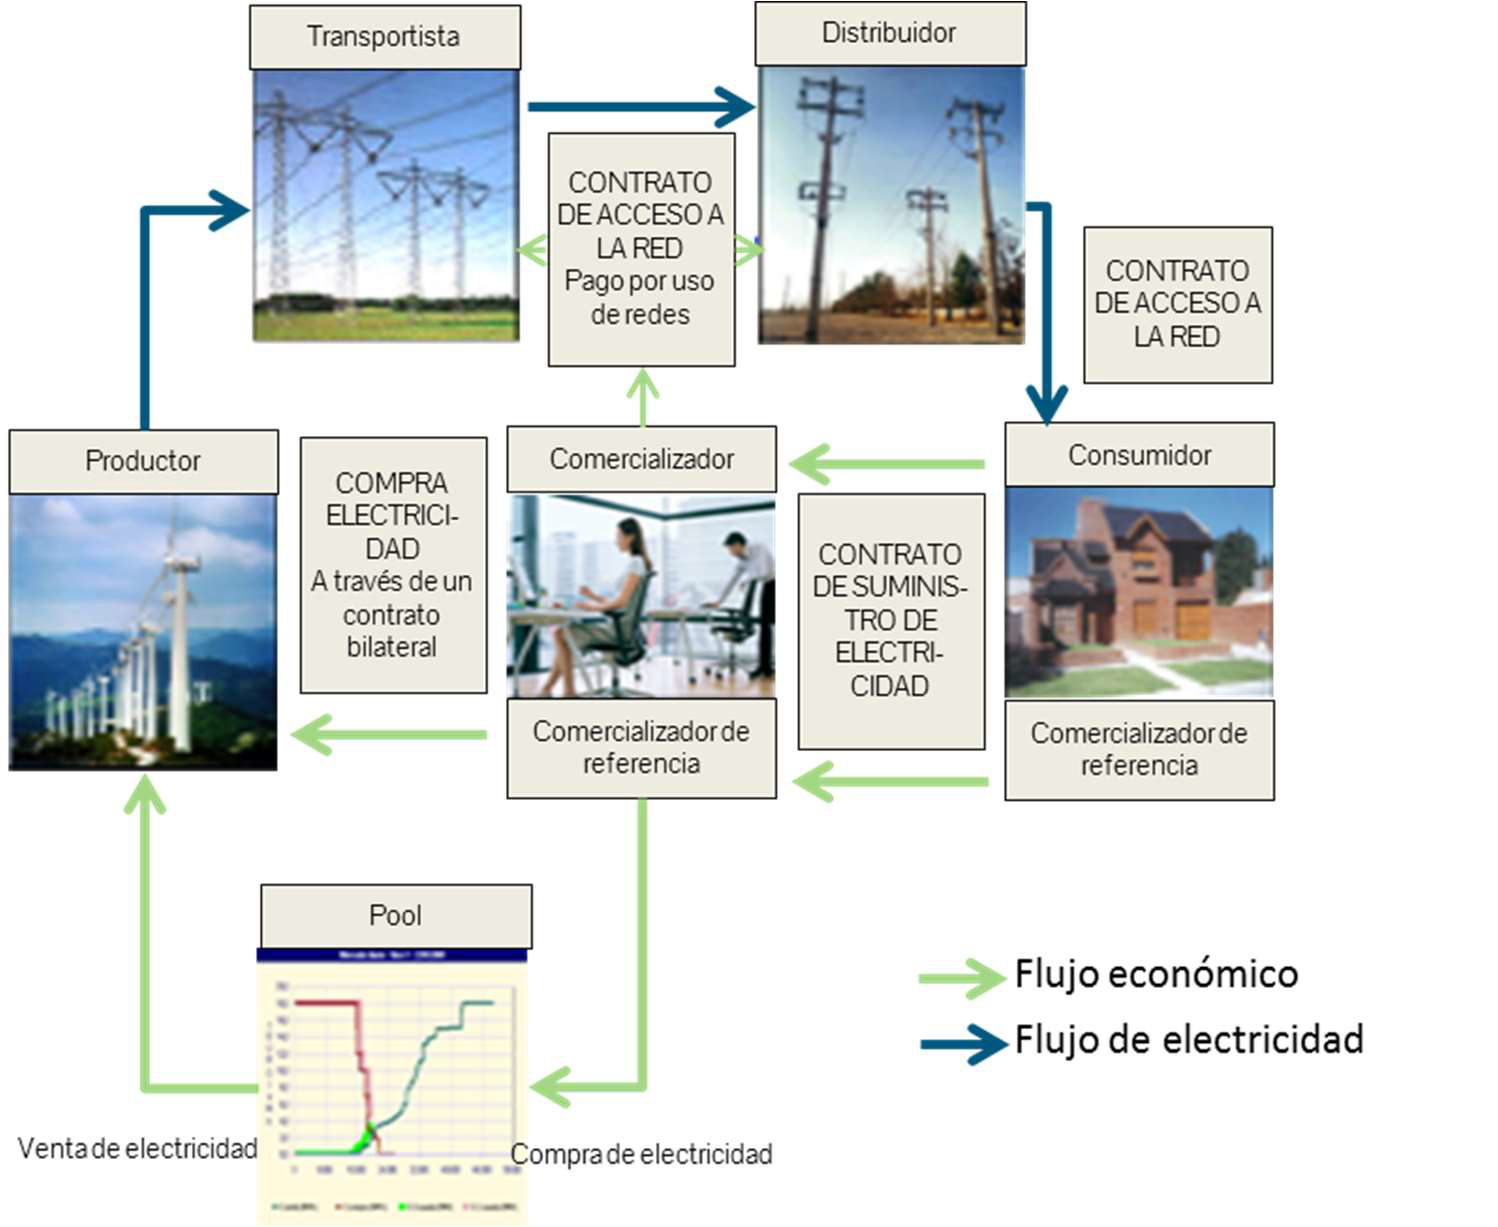
\includegraphics[width=0.7\linewidth]{res/tema4/diagramaPochoAdrikun2}
	\label{fig:diagramapochoadrikun2}
\end{figure}

\end{itemize}
\section{Mercado ibérico (MIBEL).} 
Es el resultado de una iniciativa de Portugal y España para crear un mercado conjunto entre ambos. La casación se realiza junto al resto de países europeos acoplados mediante el algoritmo Euphemia:
\begin{itemize}
	\item [-] Persigue conseguir la máxima ganancia para los vendedores, el mínimo coste
	para los compradores, las menores emisiones de CO$_{2eq}$ y optimizar el uso
	de la capacidad disponible en las interconexiones internacionales.
\end{itemize}

Además, cabe recalcar que el mercado es de tipo marginalista, es decir, que aunque haya distintas ofertas, una vez realizada la casación se paga por toda la energía al precio del último generador que ha entrado en el mercado (ordenados de menor a mayor coste de oferta).
\section{Interconexiones con el extranjero.}
Contribuyen a la seguridad y a la continuidad del suministro eléctrico y a su vez permiten una
mayor integración de las energías renovables. Si los países tuviesen capacidad de interconexión suficiente, el precio de la electricidad en ambos países seria el mismo.
\subsection{Francia.}
Actualmente hay una capacidad de interconexión 2.800 MW y se planea construir una nueva línea de interconexión en corriente continua de 2.000 MW. En 2023 se han producido diferencias de
precios entre las dos zonas el 67,2 \% de las horas
del año.
\subsection{Portugal.}
Actualmente hay una capacidad de interconexión 3.200 MW   y se planea construir una nueva línea de interconexión de 1.000 MW (se puede transmitir más energía de España a Portugal que de Portugal a España). En 2023 se han producido diferencias de
precios entre las dos zonas el 5,3 \% de las horas
del año.
\subsection{Marruecos.}
Actualmente hay una capacidad de interconexión 700 MW   y se planea construir una nueva línea de interconexión de 800 MW.
\subsection{Gestión de las interconexiones.}
La gestión de las interconexiones se realiza mediante dos metodologías en función de la interconexión entre los países:
\begin{itemize}
	\item [-] Mercados organizados o a plazos (España - Portugal)
	\item [-] Subastas de capacidad (España - Francia / España - Marruecos)
\end{itemize}
Los principales beneficiados del aumento de la capacidad de interconexión son las fuentes de energía renovables que son capaces de vender la energía que no puede ser integrada en el mercado nacional por capacidad. La península Ibérica se ve muy favorecida por esto ya que, es la región europea con mayor cantidad de energía eólica y solar.
\newpage
\section{Mercado Eléctrico.}
\subsection{Secuencia de los procesos del mercado.}
\begin{table}[H]
	\centering
	\renewcommand{\arraystretch}{1.5}
	\begin{tabular}{p{2cm}|p{2cm}|p{8cm}}
		\hline
		Día & Hora & Actividad \\
		\hline
		D-1 & 8:30 & Se plantea por la OMIE y OMIP (Portugal) el método de contrato bilateral:
		\begin{itemize}
			\item Subasta de capacidad: intercambios internacionales pactados.
			\item Mercados futuros (los agentes participantes negocian la energía que se entregará físicamente con plazos superiores a las 24 horas): no organizados y organizados.
		\end{itemize} \\\hline
		D-1 & 13:30& Subasta CESUR: se determinan las tarifas que pagaran los consumidores adscritos al PVPC.  \\\hline
		D-1 & 13:30 & Comienza el mercado diario, en la OMIE: se realiza la casación horaria donde se prepara la base de casación y se añaden los contratos bilaterales nacionales (acuerdos entre comercializadoras y generadores). \\\hline
		D-1 & 13:30 &  Se publica por el operador del sistema (REE) el programa diario base de funcionamiento donde se aplica el mercado de restricciones técnicas. El mercado de restricciones se determina en base a:
		\begin{itemize}
			\item La garantía de suministro del sistema eléctrico de potencia.
			\item Análisis de contingencias (aparición de posibles defectos).
		\end{itemize}\\\hline
		D-1 & 14:45 & Se publica el programa diario viable provisional y se aplica el mercado de servicios complementarios para los controles: Potencia - Frecuencia y Reactiva - Tensión. 
		
		Para ello, se asigna una banda secundaria de potencia activa a subir (500 MW) y bajar (400MW).
		\\\hline
		D-1 & 15:00 &  Se publica el programa diario viable definitivo.\\\hline
		D & Todo el día & Mercado intradiario y de ajustes. Se gestiona un volumen relativamente bajo.
	\begin{itemize}
		\item [-] 	En territorio nacional se realiza en 6 sesiones incluyendo el día siguiente (15:00 / 17:50 / 21:50 / 1:50 / 4:50 / 9:50).
		\item [-] En el mercado transfronterizo se realiza de manera continua.
	\end{itemize}
		\\\hline
		D & Todo el día & Programa horario final. Se realiza la gestión de desvíos mediante el mercado de restricciones técnicas del mercado intradiario y la reserva de regulación terciaria. \\\hline
	\end{tabular}
\end{table}
\newpage
\begin{landscape}
\begin{figure}
	\centering
	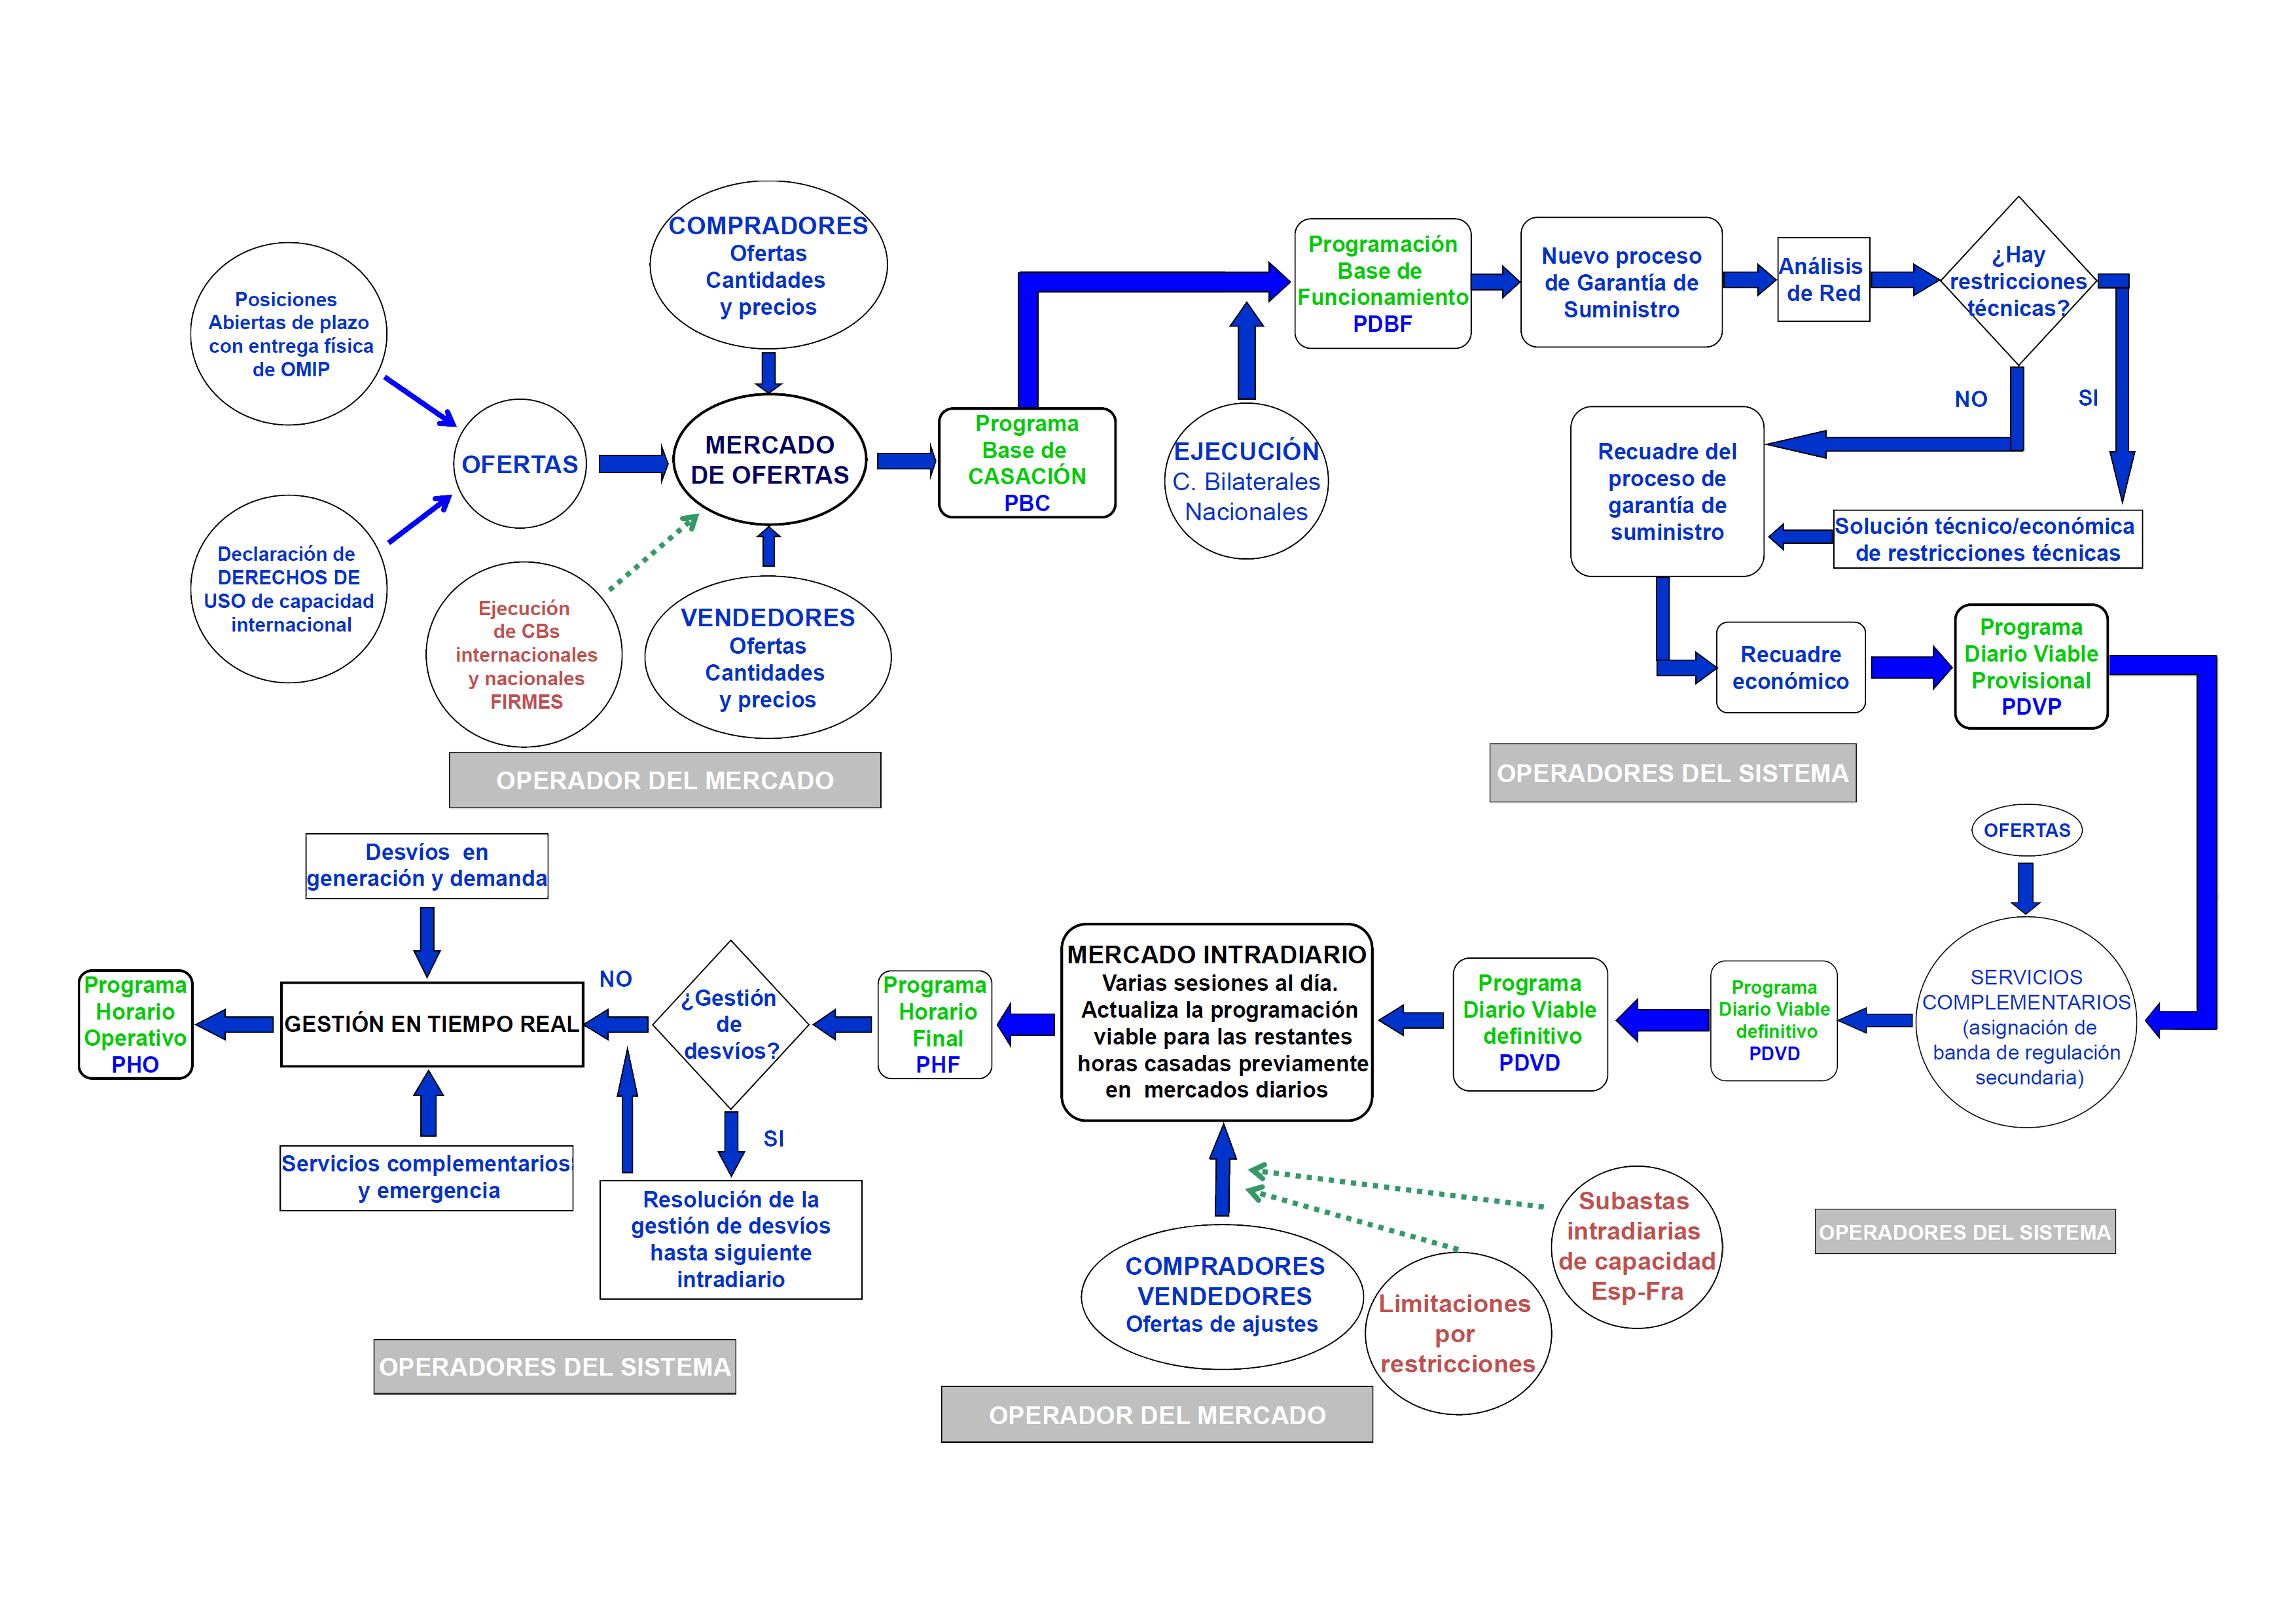
\includegraphics[width=1\linewidth]{res/tema4/funcionamientoMercado}
	\label{fig:funcionamientomercado}
\end{figure}
\end{landscape}
\newpage
\subsection{Mercados a plazo.}
Es un mecanismo que emplean tanto generadores como comercializadoras de compra al por mayor para evitar la exposición a la volatilidad de los precios del mercado diario. Estas ofertas se preparan en función de las expectativas de precios previstas.



En el mercado a plazo no organizado de contratos bilaterales (OTC) se negocian contratos mediante broker de contratos de liquidación financiera en base a sus propias reglas. En la actualidad se negocia en España un volumen de energía muy superior en los mercados a plazo
OTC que en el mercado organizado.



Un aspecto fundamental en los mercados a plazo son las subastas de capacidad donde se gestiona la capacidad comercial de intercambio para un tiempo de un año. De esta forma, se determina un único precio por la capacidad adquirida.
 
\subsection{Mercado organizado diario.}
Es un mercado físico a las 10h del día D-1 para cada una de las horas del día D y se casa al precio marginal que será el precio resultante del equilibrio entre la oferta y la demanda.
\begin{itemize}
	\item [-] \textbf{Oferentes:}
	\begin{itemize}
		\item Unidades de producción disponibles no vinculadas a un contrato bilateral físico.
		\item Comercializadores no residentes registrados como vendedores.
	\end{itemize}
	\item [-] \textbf{Demandantes:}
	\begin{itemize}
		\item Comercializadores de último recurso o de referencia.
		\item Comercializadores.
		\item Consumidores directos.
		\item Comercializadores no residentes registrados como compradores. 
	\end{itemize}
\end{itemize}

Este mercado se estructura en 24 periodos de programación equivalentes a una hora natural. 
\begin{itemize}
	\item [-] Los generadores ofertan cantidades de energía (MWh) y precio (€/MWh) para los diferentes
	períodos de programación. \textbf{Todas las unidades de producción disponibles que no estén afectas a un contrato bilateral físico
		tienen la obligación de presentar ofertas para el mercado diario.}
	\item [-] Los adquirentes ofertan cantidades y precios de compra de energía.
\end{itemize}
Se denomina unidad de producción cada una de las centrales que inyecta energía a un mismo nodo de la red.

\subsection{Proceso de casación.}
\begin{enumerate}
	\item Los agentes envían al OMEL (subdivisión del OMIE) sus ofertas para cada hora del día siguiente.
	\item La OMEL construye las curvas de oferta y demanda para cada hora.
	\item La OMEL cruza oferta y demanda para obtener el precio de mercado horario.
\end{enumerate}
 \begin{figure}[H]
 	\centering
 	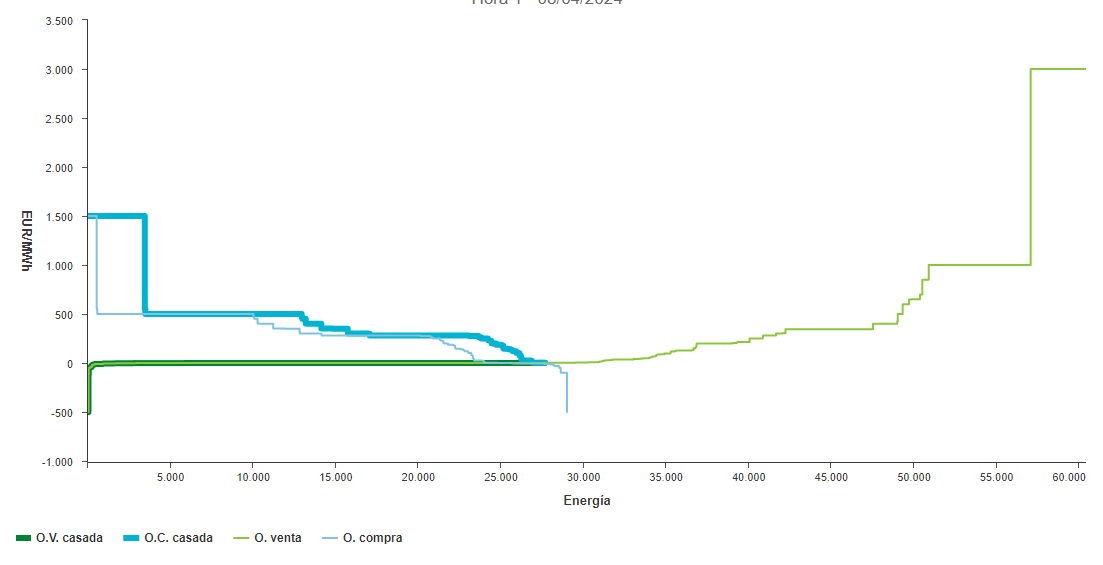
\includegraphics[width=0.7\linewidth]{res/tema4/curvasCasacion}
 	\label{fig:curvascasacion}
 \end{figure}
 \newpage
\subsection{Curva de oferta de venta de energía.}
Existen dos tipos de ofertas:
\begin{itemize}
	\item [-] Ofertas simples: Son ofertas económicas de venta de energía que los vendedores presentan para
	cada periodo horario y unidad de producción. El coste es incremental.
	\item [-] Ofertas complejas: incorporan alguna de las condiciones técnicas siguientes:
	\begin{itemize}
		\item Condición de indivisibilidad: Permite fijar en el primer tramo de cada hora un valor mínimo de potencia o de
		funcionamiento.
		\item Gradiente de carga: permite establecer la diferencia máxima entre la potencia inicio de hora y la potencia final de
		hora de la unidad de producción, lo que evita cambios bruscos en las unidades de producción
		que no pueden, técnicamente, seguir las mismas.
		\item Ingresos mínimos:  permite la realización de ofertas en todas las horas, pero respetando que la unidad de
		producción no participe en el resultado de la casación del día, si no obtiene para el conjunto
		de su producción en el día, un ingreso superior a una cantidad fija.
		\item Parada programada: permite que, si la unidad de producción ha sido retirada de la casación por no cumplir la
		condición de ingresos mínimos solicitada, realice una parada programada en un tiempo
		máximo de tres horas.
	\end{itemize}
\end{itemize}
Para realizar la casación, primero se realiza una casación con ofertas simples  y después se añaden las condiciones de las ofertas complejas.
\subsection{Coste de oportunidad fuentes de energía.}
\begin{itemize}
	\item [-]\textbf{Centrales de gas y carbón:} el coste marginal suele tender al coste marginal. Por tanto, condicionan el precio de equilibrio. 
	\item [-]\textbf{Generadores hidráulicos:} consumir agua supone el coste de oportunidad de consumir el agua en un momento futuro donde el precio de la electricidad sea mayor.
	\item [-]\textbf{Centrales nucleares y renovables:} como ofertan a coste cero tienen coste de oportunidad nulo. Y, como se ofertan a coste cero entran con prioridad en el mercado eléctrico desplazando a las energías más caras.
\end{itemize}
\begin{figure}[H]
	\centering
	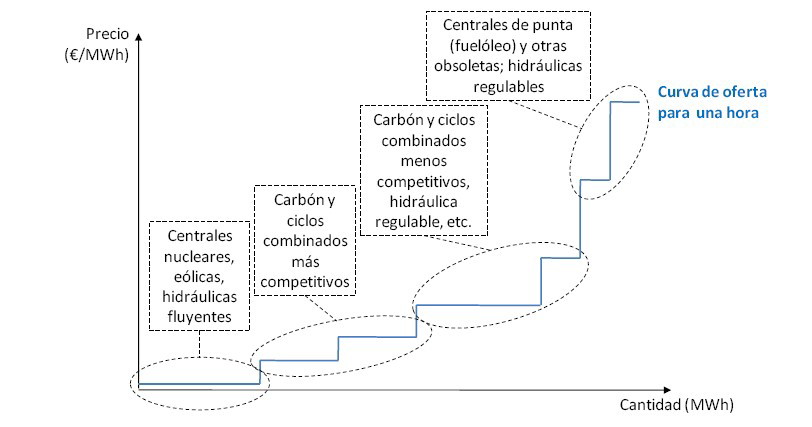
\includegraphics[width=0.7\linewidth]{res/tema4/curvaDemanda}
	\label{fig:curvademanda}
\end{figure}
\subsection{Retribuciones para amortizar costes fijos.}
Se producen a través de tres vías:
\begin{itemize}
	\item [-]\textbf{Margen del mercado:} es la diferencia entre el precio del mercado recibido y los costes variables incurridos.
	\item [-]\textbf{Pagos por capacidad o disponibilidad:} son ingresos regulados que reciben todos los generadores de ciclo
	combinado y centrales térmicas de carbón independientemente de la cantidad de energía
	producida. Los pagos por disponibilidad se configuran en función de la potencia neta instalada de la central,
	así como de un índice de disponibilidad.
	\item [-]\textbf{Servicio de interrumpibilidad:} sirve para regular el sistema desde la demanda, obligando a las grandes empresas
	que prestan este servicio a reducir su consumo en caso de necesidad, para mantener el sistema
	estable y seguro.
\end{itemize}
\subsection{Curva de demanda.}
Los distribuidores para el suministro regulado y muchos comercializadores suelen ofertar al máximo precio permitido (4.000 €/MWh) para asegurar que los consumidores obtienen la energía que demandan.
\begin{figure}[H]
	\centering
	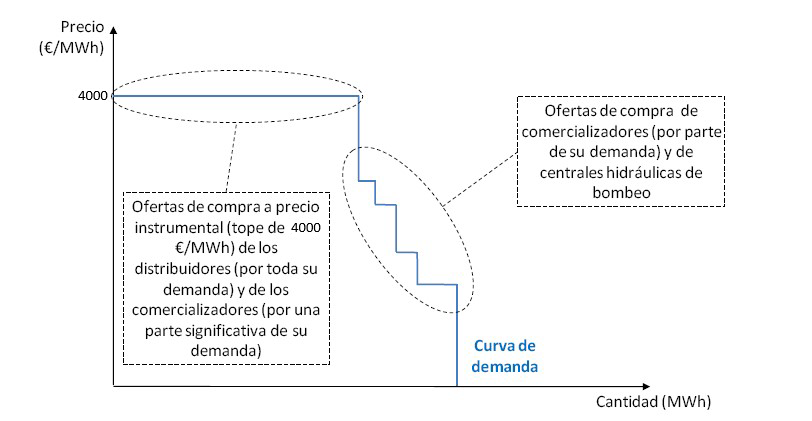
\includegraphics[width=0.7\linewidth]{res/tema4/curvaOferta}
	\label{fig:curvaoferta}
\end{figure}

\section{Mercado de restricciones técnicas.} 
El Operador del Sistema (REE) evalúa
la viabilidad técnica del programa de funcionamiento
en tiempo real (análisis de flujo de cargas) para
garantizar la seguridad y fiabilidad del suministro
en la red de transporte.


Si el resultado de la casación del mercado diario no
respeta la capacidad máxima de intercambio entre
sistemas eléctricos, o los requisitos de seguridad, el
procedimiento de solución de restricciones
técnicas modifica en el primer caso las compras o
ventas.


La solución de las restricciones técnicas constituye
una alteración no deseable del mercado, y supone
un sobrecoste derivado de dicha solución.

\begin{table}[H]
	\centering
	\renewcommand{\arraystretch}{1.5}
	\begin{tabular}{c|c}
		\hline
		Causas & Soluciones \\
		\hline
		Sobrecargas en la red & Modificación programas de energía \\\hline
		Déficit de cobertura & Limitar programas de energía \\\hline
		Límites de tensión & Teledisparos de generación \\\hline
	\end{tabular}
\end{table}
\section{Mercado de servicios complementarios.} 
Se aplica después del mercado de restricciones técnicas con el objetivo de afrontar desequilibrios de corta duración. Aumenta el coste del servicio sobre la demanda. En función de su rapidez en cuanto a regulación frecuencia-potencia se habla de:
\begin{itemize}
	\item [-] Regulación primaria (más rápida).
	\item [-] Regulación secundaria.
	\item [-] Regulación terciaria.
\end{itemize}
Los productores térmicos que necesitan varias horas de antelación para comenzar a generar
electricidad por sus prolongados procesos de arranque. No obstante, pueden ser programados para que estén
disponibles a nivel de producción más bajo y puedan ser requeridos en los mecanismos de balance cubriendo desviaciones en la programación
de la demanda u otros generadores.
\newpage
\subsection{Regulación primaria.}
Tiene como objetivo mantener la estabilidad de la frecuencia del sistema de forma automática a través de grupos generadores. Es un servicio obligatorio para los operadores no retribuidos.

El servicio debe cumplir los siguientes requisitos:
\begin{itemize}
	\item [-] Variación de carga en un 1,5\% de la potencia nominal:
	\begin{itemize}
		\item En 15s ante desvíos de frecuencia $\le$ 100 mHz
		\item Lineal entre 15 y 30s ante desvíos de frecuencia entre 100 y 200 mHz.
	\end{itemize}
\end{itemize}
\subsection{Regulación secundaria.}
Tiene como objetivo el mantenimiento del intercambio con el Área Síncrona de Europa Continental y de la frecuencia a valores programados mediante un sistema de control jerárquico mediante grupos generadores habilitados por REE. Es un servicio voluntario a cambio de una retribución.


El servicio debe realizar el seguimiento por las zonas de regulación de las variaciones de consigna de potencia activa enviadas cada 4s por el regulador maestro.
\subsection{Regulación terciaria.}
Tiene como objetivo hacer frente a desvíos imprevistos de corta duración. Es un servicio voluntario.


El servicio debe cumplir los siguientes requisitos:
\begin{itemize}
	\item [-] Tiempo de respuesta menor a 15 minutos para sustituir a la regulación secundaria.
	\item [-] La reserva mínima es aproximadamente igual al 2\% de la demanda prevista en cada hora.
\end{itemize}
\subsection{Control de tensión.}
Tiene como objetivo el mantenimiento del perfil de tensiones en los nudos de la red. Los proveedores realizan este control mediante:
\begin{itemize}
	\item Generadores (P>30MW): consigna de tensión.
	\item Transportistas: regulación en trafos de tensión y consigna ON/OFF en reactancias y condensadores.
	\item Gestores de las redes de distribución: consignas de factor de potencia.
	\item Consumidores cualificados (P>15MW): consigna factor de potencia.
\end{itemize}

Existe una parte obligatoria de mínimos así como una parte voluntaria.



Los requisitos obligatorios son:
\begin{itemize}
	\item [-] Generadores: capacidad de reactiva de $\pm 15\% P_n  $ a V$_{nominal}$.
	\item [-] Consumos: factor de potencia en la frontera $\ge0,95$ en hora punta y no capacitivo en el valle.
\end{itemize}
También existen distintas regulaciones en función de su tiempo de respuesta y se van sustituyendo unas por otras.
\begin{table}[H]
	\centering
	\renewcommand{\arraystretch}{1.5}
	\begin{tabular}{c|c}
		\hline
		Regulación & Tiempo \\
		\hline
		Primario & Milisegundos \\\hline
		Secundario & Segundos \\\hline
		Terciario & Minutos \\\hline
	\end{tabular}
\end{table}
\subsection{Gestión de desvíos.}
Se repite la casación para corregir las previsiones por una predicción inexacta del viento o una avería de una central con el objetivo de afrontar desequilibrios de $>$300MW a través de los proveedores. Es un servicio voluntario.

\section{Precio medio final.} 
En el mercado eléctrico aparecen los siguientes conceptos en la tarifa eléctrica:
\begin{itemize}
	\item [-]\textbf{Coste de producción (35\%):} determinado en el mercado de producción
	\item [-]\textbf{Costes regulados (40\%):} 
	\begin{itemize}
		\item Los accesos y peajes por transporte de energía eléctrica determinados por la
		CNMC.
		\item Los accesos y peajes por distribución de energía eléctrica determinados por la
		CNMC. El precio será diferente según el horario de consumo (punta/valle/llano).
		\item Los costes de comercialización: Margen de comercialización de las empresas
		comercializadoras.
		\item Los costes permanentes del sistema engloban:
		\begin{itemize}
			\item  Desarrollo del suministro de electricidad en Baleares, Canarias, Ceuta y Melilla.
			\item  Costes de mantenimiento de las actividades del Operador del Mercado (OMIE).
			\item Costes de mantenimiento de las actividades del Operador del Sistema (REE).
			\item Costes de mantenimiento de las actividades de la CNMC.
			\item Bono Social (25\% de descuento).
			\item Pagos por capacidad y servicio de interrumpibilidad.
		\end{itemize}
	\end{itemize}
	\item [-]\textbf{Costes de diversificación y seguridad de abastecimiento (2\%):}
	\begin{itemize}
		\item Retribución a la producción de las energías renovables.
		\item Los costes asociados a centrales nucleares que no se llegaron a poner en marcha.
		\item Los costes derivados de la financiación del segundo ciclo del combustible nuclear (coste ya transferido a las centrales nucleares).
		\item Los costes de stock estratégico del combustible nuclear (residuos en el extranjero).
	\end{itemize}
	\item [-]\textbf{Impuestos (23\%):} compuestos por el IVA y el impuesto especial sobre la electricidad.
	
\end{itemize}
\begin{figure}[H]
	\centering
	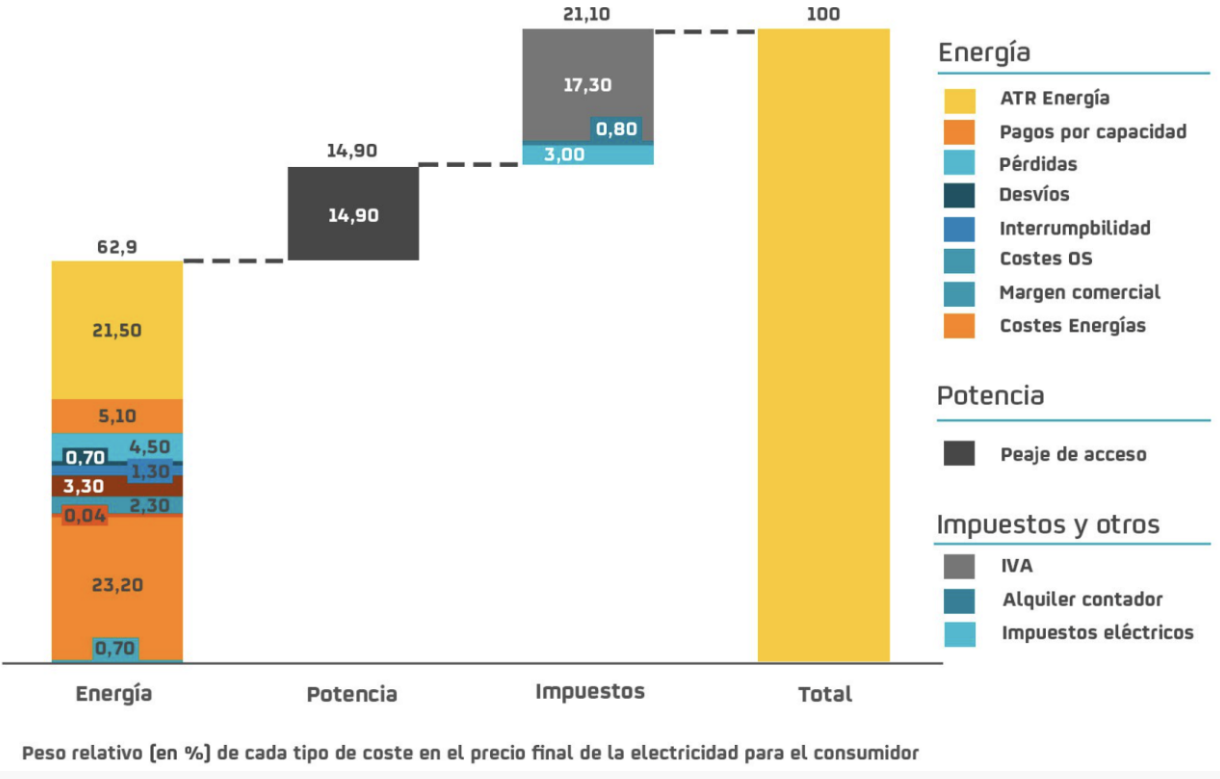
\includegraphics[width=0.7\linewidth]{res/tema4/pvpc}
	\label{fig:pvpc}
\end{figure}
\newpage
\section{Programación de la generación de electricidad.}
La electricidad se planifica a largo plazo para tener en cuenta escenarios de crecimiento del PIB, de capacidad de interconexión y periodos de mantenimiento.
\subsection{Curva acumulada de demanda anual.}
Para estudios de planificación a más largo plazo tiene utilidad emplear una curva ordenada de la demanda anual para asegurar que el parque de generación pueda suministrar la demanda máxima. Se obtiene sumando para cada nivel de potencia demandada el nº de horas en que dicha potencia
se ha igualado o superado a lo largo del año. El área que queda debajo de la curva es la energía
demandada Eda (MWh).
\begin{figure}[H]
	\centering
	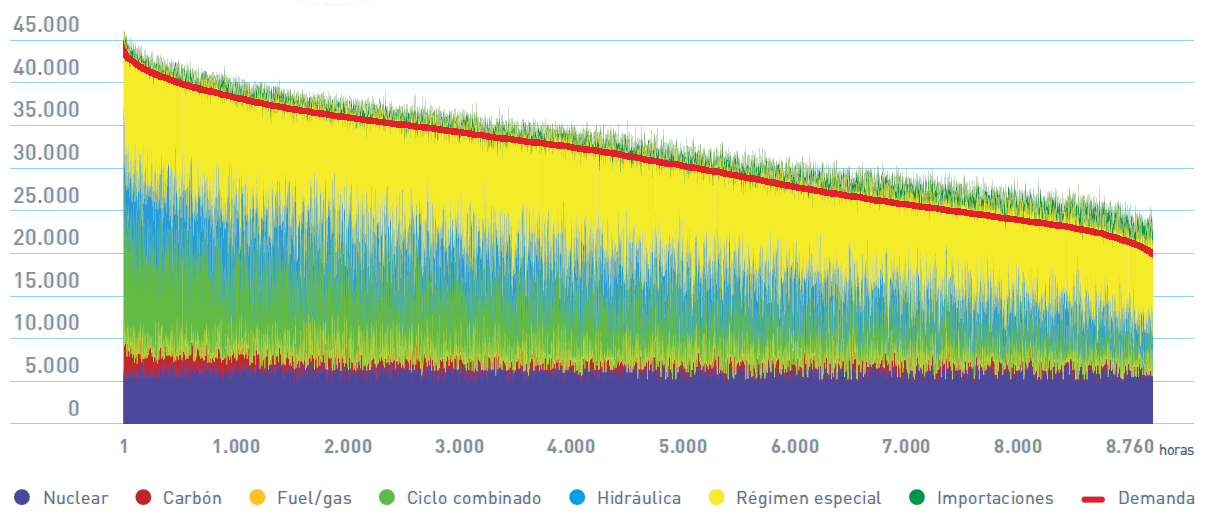
\includegraphics[width=0.7\linewidth]{res/tema4/curvaDemandaAnual}
	\label{fig:curvademandaanual}
\end{figure}
Si se divide esta curva por el número de horas en un año 8760 se obtiene una distribución de probabilidad acumulada. 



Para cubrir esta demanda de forma óptima (mínimo coste) habría que utilizar cada una de las tecnologías óptimas para cada uno de los rangos de horas de
funcionamiento. De esta forma, se configura el parque de generación para cubrir estas necesidades.
\begin{figure}[H]
	\centering
	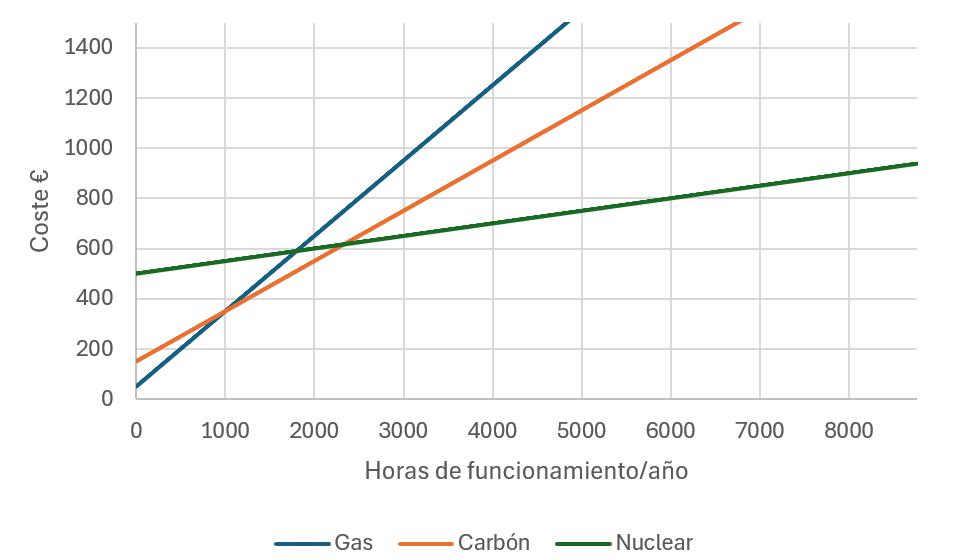
\includegraphics[width=0.7\linewidth]{res/tema4/curvaCostes}
	\label{fig:curvacostes}
\end{figure}

\subsection{Parámetros principales curva de demanda.}
\begin{itemize}
	
	\item [-] \textbf{Energía demandada (EDa) (MWh):} es el área bajo la curva de demanda anual.
	\item [-] \textbf{Potencia demanda media anual ( P$_{D_{med}}$) (MW):} 
	\[P_{D_{med}}[MW]=\frac{EDa[MWh]}{8760[h]}\]
	\item [-] \textbf{Demanda máxima ( P$_{D_{max}}$) (MW):} es el pico de la demanda que se alcanza en el periodo de tiempo
	analizado.
	\item [-] \textbf{Demanda mínima ( P$_{D_{min}}$) (MW):} es el valle de la demanda que se alcanza en el periodo de tiempo
	analizado.
	\item [-] \textbf{Factor de carga (f$_{car}$) o índice cobertura:} Es el criterio para evaluar la necesidad de potencia en el sistema
	eléctrico es el índice de cobertura. Según el criterio del operador del sistema eléctrico, este índice
	debería ser igual o superior a 1,1.
	\[f_{car}=\frac{P_{D_{med}}[MW]}{P_{D_{max}}[MW]}\]
	\item [-] \textbf{Potencia conectada (P$_{con}$):} es la suma de las potencias contratadas por todos los abonados. Es mucho menor a la potencia máxima. 
	\item [-] \textbf{Factor de simultaneidad (s):} 
	\[s=\frac{P_{D_{max}}[MW]}{P_{con}[MW]}\]
\end{itemize}
\subsection{Curva acumulada de generación anual.}
Es la curva que se obtiene en barras de la central. Equivale a sumarle a la curva de generación las pérdidas.
\subsection{Parámetros principales curva de generación.}
\begin{itemize}
	\item [-]\textbf{Energía generada (EGa) (MWh):} es el área bajo la curva de generación anual.
	\item [-]\textbf{Potencia generada media anual (P$_{G_{med}}$) (MW):} 
		\[P_{G_{med}}[MW]=\frac{EGa[MWh]}{8760[h]}\]
	\item [-]\textbf{Potencia generada máxima (P$_{G_{max}}$) (MW):}  es el pico de la generación que se alcanza en el
	periodo de tiempo analizado.
	\item [-]\textbf{Potencia generada mínima (P$_{G_{min}}$) (MW):}  es la mínima generación que se alcanza en el periodo
	de tiempo analizado.
	\item [-]\textbf{Potencia instalada (P$_{inst}$) (MW):}  es la suma de las potencias nominales de todos los grupos que
	componen el parque de generación.
	\item [-]\textbf{Potencia disponible (P$_{disp}$) (MW):}  es la diferencia entre la potencia instalada y la suma de las de
	los grupos indisponibles por mantenimiento, revisión o avería.
	\item [-]\textbf{Potencia no disponible (P$_{no\ disp}$) (MW):} es la potencia de los generadores que se encuentran
	fuera de servicio por mantenimiento programado, mantenimiento correctivo o
	que no pueden funcionar a su potencia nominal por falla parcial.
	\item [-]\textbf{Reserva de potencia (PG) o Factor de reserva (fr):}
	\[fr=\frac{P_{disp}[MW]}{P_{max}[MW]}\]
	\item [-]\textbf{Factor de capacidad (FC):}  Es un factor adimensional en base anual que se usa para generación y da una idea de cuanto se está utilizando
	la capacidad de generación de un conjunto de centrales.
	\[FC=\frac{P_{G_{med}}[MW]}{P_{G_{nom}}[MW]}\]
	\item [-]\textbf{Horas de utilización anual (TU) (h):} Definido como el tiempo en que el generador debería funcional a su PGnom de manera continua, para que esas
	condiciones de energía producida sea igual a la energía producida anual EGa.
	\[TU [h]=FC\cdot 8760 [h]\]
\end{itemize}
\newpage
\section{Reserva de potencia.} 
Se distinguen tres tipos de reserva según el tiempo de acceso (intervalo de tiempo entre la aparición de la necesidad y el instante donde ha sido cubierta):
\begin{itemize}
	\item [-]\textbf{Reserva rodante:} está constituida por la capacidad de producción de los grupos en
	funcionamiento y que en un instante determinado no es utilizada (la carga restante hasta su potencia nominal). 
	\item [-]\textbf{Reserva rápida:} Está constituida por la suma de las potencias de los grupos de arranque
	rápido (hidráulicos y turbinas de gas) que se encuentran parados. Su tiempo de arranque varía
	entre 2 y 10 minutos.
	\item [-]\textbf{Reserva lenta:} La integran los grandes grupos de las centrales térmicas de carbón y nucleares
	desconectadas de la red y que tienen unos tiempos de arranque de varias horas.
\end{itemize}
La reserva se determina en función de las probabilidades de avería de los distintos generadores.
\subsection{Características estáticas.}
Se relacionan con la capacidad de producir energía para cada nivel de potencia. 
\begin{itemize}
	\item [-]Las centrales térmicas pueden funcionar teóricamente entre la potencia máxima y la potencia de
	mínimo técnico. Tienen, en principio, una disponibilidad de energía primaria ilimitada.
	\item [-] Las centrales hidráulicas pueden ver afectada su producción por variaciones en la altura del salto y
	por las disponibilidades de agua de la cuenca. Tienen mayores restricciones.
\end{itemize}
\subsection{Características dinámicas.}
Se refieren a la capacidad de variar el valor de la potencia instantánea producida. La velocidad de respuesta es mucho mayor en las centrales hidráulicas y de ciclo combinado que
en las centrales térmicas de carbón y nucleares a causa de la inercia térmica de las calderas y reactores. Otra consideración dinámica es el tiempo de arranque mínimo, de gran importancia en
situaciones de emergencia en la red.

\subsection{Secuenciamiento óptimo de grupos.}
Debido a los tiempos de parada programados se requiere que a lo largo del año
hayan entrado en funcionamiento un número de centrales mayor del que sería necesario. Por tanto, a lo largo del año se necesita acudir a la reserva
lenta de potencia durante los periodos de revisión.
\section{Costes de generación (LCOE).}
El método LCOE (leverised cost of electricity) es un método empleado para comparar distintas tecnologías de generación y evaluar su viabilidad económica. Indica cuanto dinero ha costado generar 1kWh a lo largo de un año o su vida útil.
\[LCOE=\frac{\text{Costes totales de la plan} [\euro{}]}{\text{Energía total generada}[kWh]}\]
Una central con un LCOE bajo es más rentable y competitiva en términos de costo de
generación de energía a lo largo de su vida útil.
\[LCOE=\text{Coste de inversión}+\text{Coste operación}+\text{Coste combustible}+\text{Coste CO}_2+\text{Coste desmantelamiento} \left[\frac{\euro}{MWh}\right]\]
Factores que afectan al LCOE:
\begin{itemize}
	\item [-]\textbf{Costos de inversión inicial:} los costos asociados a la construcción y puesta en marcha del
	proyecto.
	\item [-]\textbf{Costos de operación y mantenimiento:} los costos recurrentes asociados a la operación y el
	mantenimiento del proyecto a lo largo de su vida útil.
	\item [-]\textbf{Costos asociados a los combustibles:} los costos relacionados con el
	suministro de combustibles.
	\item [-]\textbf{Costos asociados a las emisiones de dióxido de carbono:} vienen impuestos por normativa europea.
	\item [-]\textbf{Costos de desmantelamiento:} de la central tras su vida útil.
	\item [-]\textbf{Vida útil del proyecto:} la duración estimada del proyecto.
	\item [-]\textbf{Tasa de descuento:} la tasa utilizada para descontar los flujos de efectivo futuros y llevarlos a valor
	presente.
	\item [-]\textbf{Eficiencia de la tecnología utilizada:} la eficiencia con la que la tecnología utiliza los recursos
	energéticos disponibles. 
\end{itemize}
\subsection{Comparativa de costes.}
\begin{figure}[H]
	\centering
	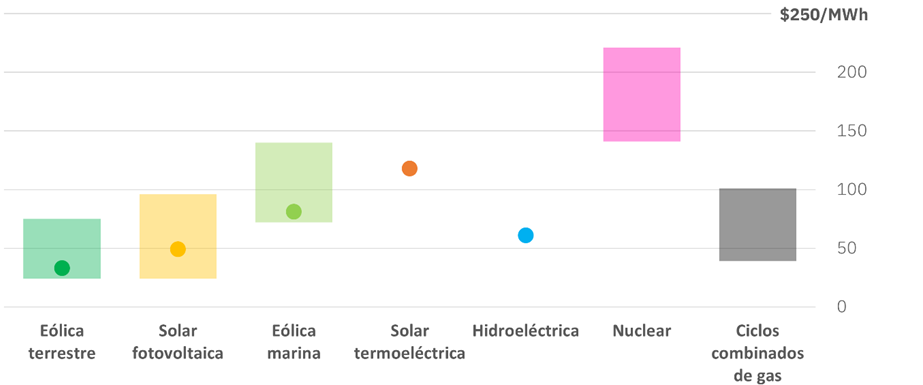
\includegraphics[width=0.7\linewidth]{res/tema4/lcoe}
	\label{fig:lcoe}
\end{figure}

\subsection{Coste de inversión o fijo.}
Es un coste constante e independiente del número de horas de utilización anual de la central.  Estos costes se reparten de forma constante durante toda la vida de la central, mediante pagos
anuales.
\[\text{Coste inversión} \left[\frac{\euro}{MWh}\right]=
\frac{
	\text{Inversión inicial}\left[\frac{\euro}{MWh}\right] \cdot P_e [MWe]\cdot(1+i)^r\cdot\frac{i\cdot(1+i)^{n-r}}{(1+i)^{n-r}-1}[\frac{1}{\text{año}}]
	}{P_e [MWe]\cdot8760\left[\frac{h}{año}\right]\cdot FC }\]
	
Donde:
\begin{itemize}
	\item $i$ es el tipo de interés.
	\item $r$ es el periodo de pago sin intereses.
	\item $n$ es el horizonte económico del proyecto.
\end{itemize}
\subsection{Costes variables.}
Dependen del número de horas de utilización anual e incluyen:
\begin{itemize}
	\item [-] Coste del combustible consumido.
	\item [-] Coste de operación.
	\item [-] Coste por las emisiones de CO$_2$.
\end{itemize}
\[C_v=C_{OyM}+C_{Comb}+C_{CO_2} \left[\frac{\euro}{MWh}\right]\]
\subsection{Coste total.}
El coste total representa el gasto total anual necesario para mantener en servicio la central
produciendo una determinada cantidad de energía anual, durante un número de horas. Se pueden representar mediante la ecuación de una recta.
\[C_t=C_f+C_v \left[\frac{\euro}{MWh}\right]\]
\subsection{Indices principales.}
\begin{itemize}
	\item [-] Coste total anual de generación por MW instalado:
	\[C_p=\frac{C_t}{P_{inst}} \left[\frac{\euro}{MW}\right]\]
	\item [-] Coste específico:
	\[C_e=\frac{C_t}{P_{inst}\cdot horas} \left[\frac{\euro}{MWh}\right]\]
\end{itemize}
\section{Aspectos técnicos de la producción de energía.} 
Desde 1985, REE mide la Calidad de Suministro de la red de transporte en base a una serie de indicadores
calculados todos ellos a partir de la energía no suministrada (ENS) a consumidores finales debida a incidencias
iniciadas en la red de transporte.





El principal indicador utilizado por REE es el tiempo de interrupción medio (TIM).
\[TIM = \frac{60\cdot ENS}{\text{Demanda anual}} [min]\]
\begin{table}[H]
	\centering
	\renewcommand{\arraystretch}{1.5}
	\begin{tabular}{cccc|ccc}
		\hline
		 & &&ENS(MWh)&&&TIM (minutos) \\\hline
		Año&Península &Baleares&Canarias&Península &Baleares&Canarias \\\hline
		2016&78  &0,3  &46&0,16&0,03&27,5 \\\hline
		2017&60  &33   &47&0,13&2,88&2,75 \\\hline
		2018&250 &38   &63&0,52&3,27&3,77 \\\hline
		2019&47  &1    &2,6&0,10&0,09&155,5 \\\hline
		2020&95  & 4   &65&0,21&0,47&4,29 \\\hline
	\end{tabular}
\end{table}
Además, en la calidad del suministro es relevante mantener unos margenes de tensión y una cierta calidad en la onda de tensión.